\documentclass[letterpaper,twoside,11pt,headings=small]{scrartcl}

\PassOptionsToPackage{hang,small}{caption}
\usepackage[margin=1in]{geometry}
\usepackage{amsmath,amsfonts,amssymb,amsthm}
\usepackage{graphicx}
\usepackage[english]{babel}
\usepackage{subfig}
\usepackage{fancyvrb}
\usepackage{booktabs}
\usepackage{tabularx}
\usepackage{chappg}
\usepackage{xspace}
\usepackage{scrpage2}
\usepackage{pgf,tikz}
\usetikzlibrary{calc}
\usetikzlibrary{arrows}
\usepackage{ulem}
\normalem
\usepackage{fontspec}
\usepackage{xunicode}
\usepackage{xltxtra}
\defaultfontfeatures{Mapping=tex-text}
\setromanfont[Ligatures={TeX}]{Times New Roman}
\setsansfont[Ligatures={TeX}]{Helvetica Neue}
\setmonofont[Scale=MatchLowercase]{Menlo}
\usepackage{todonotes}
\usepackage{paralist}

\newcommand{\basetitle}{TWC: Medium: Collaborative: Automated Reverse Engineering of Commodity Software}
\newcommand{\thetitle}{\basetitle\xspace}
\newcommand{\dynamicsys}{\textsc{PANDA}\xspace}
\newcommand{\challenge}[1]{\paragraph{Research Challenge:} \emph{#1}}

\pagestyle{scrheadings}
\clearscrheadfoot
\lohead{\thetitle}
\rohead{\pagemark}
\lehead{\thetitle}
\rehead{\pagemark}
\setheadsepline{0.5pt}
\setfootsepline{0pt}
\setkomafont{pageheadfoot}{\sffamily\fontsize{9}{9}\selectfont}
\setkomafont{pagenumber}{\sffamily\fontsize{9}{9}\selectfont}

\usepackage[unicode,bookmarks,colorlinks,breaklinks,pdftitle={\basetitle},pdfauthor={}]{hyperref}
\hypersetup{linkcolor=black,citecolor=black,filecolor=black,urlcolor=black}

\begin{document}

\pagenumbering[B]{bychapter}

{\sffamily\bfseries
\begin{center}
\fontsize{16}{16}\selectfont Project Summary

\fontsize{13}{13}\selectfont \thetitle
\end{center}
\label{sec:summary}
}

Software, including common examples such as commercial applications or
embedded device firmware, is often delivered as closed-source binaries.  While
prior academic work has examined how to automatically discover vulnerabilities
in binary software, and even how to automatically craft exploits for these
vulnerabilities, the ability to answer basic security-relevant questions about
closed-source software remains elusive.  For instance, ideally one would like
to know whether software contains malicious functionality; whether it contains
obfuscated code or protocols indicative of malicious behavior; what security
properties does this software intend to provide; and, whether one can
recognize when software is deviating from normal, intended behavior at
runtime.

This project aims to provide algorithms and tools for answering these
questions. Leveraging prior work on emulator-based dynamic analyses, we
propose techniques for scaling this high-fidelity analysis to capture and
extract whole-system behavior in the context of embedded device firmware and
closed-source applications.  Using a combination of dynamic execution traces
collected from this analysis platform and binary code analysis techniques, we
propose techniques for automated structural analysis of binary program
artifacts, decomposing system and user-level programs into logical modules
through inference of high-level semantic behavior.  This decomposition
provides as output an automatically learned description of the interfaces and
information flows between each module at a sub-program granularity.

In addition to a \emph{structural} understanding of software, a reverse
engineering task may require a \emph{semantic} understanding as well. Building
on emulation-based dynamic analysis and structural decomposition as a
foundation, we will develop automated techniques for producing high-level
summaries of whole system executions and software components, allowing reverse
engineers to quickly obtain human-readable labels like ``encryption'' or ``file
parsing'' for modules and functions.

Finally, as an example application of our framework for whole-system
understanding, we propose techniques for automating the reverse engineering
and fuzz testing of encrypted network protocols commonly used by malware to
obfuscate their communication with command-and-control servers.  However, we
envision that the techniques and analysis platform developed as part of this
project will find wide application in the area of automated reverse
engineering and behavioral understanding of closed-source software.

\paragraph{Intellectual Merit.} Reverse engineering is a critical capability
for understanding and responding to software-borne threats, and can enable
deep system understanding towards automated hardening of existing
closed-source platforms.  However, reverse engineering currently entails the
training of highly-skilled security professionals, as well as significant
manual effort, both processes that do not scale to meet the current needs of
industry and government.  The automated techniques and tools we will develop
in the course of this research will lay the groundwork for meeting this need,
as well as enable new automatic hardening and threat response capabilities.

\paragraph{Broader Impacts.} The research proposed herein will have a
significant impact outside of the security research community.  We will
incorporate the research findings of our program into our undergraduate and
graduate teaching curricula, as well as in extracurricular educational efforts
such as Capture-the-Flag that have broad outreach in the greater Boston and
Atlanta metropolitan areas.  The close ties to industry that the collective
PIs possess will facilitate transitioning the research into practical
defensive tools that can be deployed into real-world systems and networks. As
a result, the program will have broad impact on both the training of
next-generation cybersecurity professionals as well as the advancement of
defensive tool capabilities in operational environments.

\newpage
\pagenumbering[D]{bychapter}
\setcounter{page}{1}

{\sffamily\bfseries
\begin{center}
\fontsize{16}{16}\selectfont Project Description

\fontsize{13}{13}\selectfont \thetitle
\end{center}
}

\section{Research Overview}
\label{sec:overview}

Software is predominantly distributed in the form of closed-source software,
from embedded device firmware to full-fledged commercial applications.  While
distribution of software as binary artifacts is convenient for developers and
provides a measure of protection for intellectual property rights, it is also
a significant obstacle to improving the security of our systems and the
Internet.  Traditional approaches to program understanding and security
analysis are greatly impeded by the loss of metadata such as debugging
symbols, type annotations, and structure that occurs when source code is
compiled into binary form.  Therefore, many analysis and hardening techniques
developed under the assumption of availability of source code are ineffective
when this assumption is violated.

In recognition of this problem, prior academic work has investigated binary
analyses of closed-source software to recover this
metadata~\cite{lee:ndss2011:tie}, identify vulnerabilities~\cite{kruegel:acsac2004:kernel}, harden existing
platforms~\cite{baliga:gibraltar,chipounov:asplos2011:s2e}, and even to automatically generate
exploits for detected vulnerabilities~\cite{kruegel:sec2005:mimicry,avgerinos:ndss2011:aeg,schwartz:sec2011:q,cha:oakland2012:mayhem}.
However, answering basic security-relevant questions about closed-source
software remains difficult.  For instance, ideally one would like to be
able to ascertain%
\begin{inparaenum}[\itshape a\upshape)]
    \item whether software contains hidden malicious functionality;
    \item whether it contains obfuscated code or protocols indicative of malicious behavior;
    \item what security properties does this software intend to provide; and,
    \item whether one can recognize when software is deviating from normal, intended behavior at runtime.
\end{inparaenum}

Recent discoveries of embedded backdoors in commodity devices illustrate this
point well.  In several cases over the past few years, hidden backdoors with
hardcoded authentication credentials have been found in devices such as
routers~\cite{heffner:dlink-dir100} and printers~\cite{cert:hp-backdoor} that
are intended to allow for remote administration by support staff.  However,
these backdoors could also easily be abused by attackers that either privately
discover these backdoors or exploit them after disclosure to the public.
Identifying the presence of such backdoors entails a painstaking process of
manual reverse engineering by skilled analysts, and there is currently no
systematic, automated means to accomplish this on the scale required to
achieve assurance that an organization's deployed devices are free of such
vulnerabilities.

In general, the capability to automatically and efficiently reverse engineer
closed-source software to produce a high-level understanding of its security
characteristics and runtime behavior is highly desirable.  To that end, this
project aims to develop this capability through novel research and development
of a dynamic analysis framework for this specific purpose.  In particular, we
propose to achieve the following goals:%
\begin{inparaenum}[\itshape a\upshape)]
    \item scalable whole-system dynamic analysis of closed-source software;
    \item structural decomposition and inference of software module boundaries and interfaces at a sub-process granularity;
    \item semantic understanding of the behavior of these modules through concise behavioral summaries; and,
    \item concrete applications on top of this foundation, such as automatic identification of encrypted protocol implementations in closed-source software.
\end{inparaenum}

In the following, we elaborate upon the main research thrusts of this project,
enumerate specific research challenges that will be overcome, and summarize
the anticipated project outcomes and deliverables.

% \subsection{Project Goals and Scope}
% \label{sec:overview:goals}

\subsection{Embedded Firmware Emulation}
\label{sec:overview:firmware}

For the vast majority of embedded platforms, there exists no public emulator
that can run the native firmware. This poses a major hindrance to analysis of
embedded software, because analyses must either be purely static, or the
embedded device must support debugging instrumentation (e.g., JTAG). However,
adding support to emulators for specific (undocumented) platforms is extremely
time-consuming and performing this task manually cannot hope to scale to the
thousands of embedded platforms that exist today.

We propose instead to tackle the core problem of running embedded firmware in
an emulator by automating the creation of emulated peripherals. To do so we
will make use of the key insight that many properties of the underlying
hardware can be derived from the way the firmware interacts with it. Our goal
is to reduce the amount of manual labor needed to support emulation of a new
embedded platform to a minimum.

\challenge{Can we accurately infer the range of expected values and
behavior for an embedded peripheral?}

To model an embedded peripheral, one must be able to answer a number of
questions about its behavior. How should it respond when the CPU reads a value
at a memory-mapped I/O range? When should its interrupts fire? If the device
supports DMA, when and what should it read and write to main memory? We
believe that for many peripherals, these questions can be answered by
analyzing the firmware's interactions with it, and we plan to build a system
that automates this task.

\challenge{Once we have a model of the peripheral, can we automatically
generate an emulated device that operates well enough to run the embedded firmware?}

Having derived a specification for the behavior of an embedded peripheral, we
would like to avoid having to manually write code that implements the behavior
in an emulator. Thus, as an additional research task we will need to develop
ways of automatically generating code for \dynamicsys~\cite{panda}, our
existing platform for scalable and precise dynamic analysis, that emulates the
peripheral.

\challenge{Is the resulting emulation correct?}

Because our models will be derived from the embedded firmware, there may be
aspects that do not match the real hardware. This raises the question of how
we can be confident that tests carried out on our emulator reflect reality.
Thus, to obtain confidence that our emulation is accurate, we plan to design a
test regimen that compares real device execution to emulator behavior.

\subsection{Structural Decomposition}
\label{sec:overview:structure}

A second thrust of this project will be the development of novel techniques
for structurally decomposing closed-source software into its constituent
modules.  Building upon the scalable, whole-system analysis platform provided
by \dynamicsys, structural decomposition entails discovery of not only the
boundaries of modules that comprise an otherwise opaque binary artifact, but
also the interfaces and information flows between these modules.  We envision
accomplishing this through the use of architecture-specific domain knowledge
and precise static and dynamic data flow analysis that characterizes not only
the flows themselves, but also the range of possible values that can flow along
a path.

In addition, we will develop novel dynamic invariant inference techniques that
allow our system to characterize and establish bounds on the normal behavior
of individual modules.  This will enable the capability to detect deviations
from normal behavior during runtime, as well as the potential to infer high-level
semantic behavior from low-level features.

As a final component of this thrust, we will investigate efficient binary
rewriting techniques to implement inline detection of deviations from inferred
invariants, and optional enforcement of normal behavior.

Achieving these goals requires surmounting several key research challenges.

\challenge{Can we reliably recover module boundaries from binary artifacts?}

Distinguishing module boundaries is a daunting task in and of itself.  However,
prior work has demonstrated that such techniques are possible in the case of
user-level applications~\cite{bittau:nsdi2008:wedge}.  We plan to extend these
techniques using a novel set of program and architectural features to a whole-system
setting, enabled by our dynamic analysis platform.  The intuition behind our
approach is that software engineering practices dictate modularization of
programs and system composition, and that this structure remains present,
though obfuscated, in derived binary artifacts.

\challenge{Can we achieve high coverage of realistic system inputs to infer useful invariants?}

Critical to any dynamic analysis approach is the question of coverage. Despite
their advantages in terms of precision, without careful consideration, dynamic
analyses can fail to exercise critical sections of code that could lead to
missed vulnerabilities and exploits, or an incomplete characterization of
program behavior in the context of this project.  To ameliorate this risk, we
plan to incorporate symbolic execution and automated theorem proving -- e.g.,
SMT solvers~\cite{demoura:tacas2008:z3,zheng:fse2013:z3str} -- to generate new test inputs from
seed inputs that broaden the coverage of our dynamic analysis.

\challenge{Can we recover useful higher-level semantic information from inferred invariants?}

Dynamic invariant inference has been demonstrated to be highly useful in
highlighting important assumptions of low-level program characteristics, such
as function pre- and post-conditions.  However, it is an open question as to
whether low-level invariants can be used to infer higher-level semantics with
respect to program behavior.  Overcoming this challenge will require careful
selection of the invariants that correspond to different high-level data
structures and known classes of software behaviors.  We plan to derive a
systematic mapping between classes of invariants through a combination of
domain knowledge and automated learning from known examples of different
module classes.

\subsection{Summarizing Software Execution}
\label{sec:overview:autosummary}

Building on the low-level structural decomposition and dynamic invariant
detection work described in the previous section, we will examine the question
of whether \emph{high-level semantic summaries} of execution can be
automatically created for previously unseen software. These kinds of summaries
could be enormously valuable for explicating the behavior of software, and
could vastly speed up the work of reverse engineering. For example, by looking
at a summary of program behavior that includes ``input parsing,'' a reverse
engineer can immediately know where he should focus his efforts to find flaws
in input handling.

\challenge{What should high-level descriptions of execution look like?}

Although we have given a brief example of what a portion of a summary might
look like, it is difficult to generalize this to arbitrary execution. As we
argue in Section~\ref{sec:research:autosummary}, handwritten labels are likely
to be inaccurate or incomplete, and in any case are difficult to scale to
a large software corpus. Instead we will investigate automatic semantic
labeling by training on open source software, for which high-level semantic
information such as comments, variable names, and documentation is available.

\challenge{Can these high-level summaries be automatically learned?}

Given a corpus of existing software that is somehow annotated with its
high-level semantics, it is not obvious that there is a way to classify the
execution of new software. We propose to investigate using dynamic features of
the software as it executes in order to generate a set of observations for use
in machine learning. This is a natural fit for implementation within
\dynamicsys, which supports easily instrumenting whole-system execution on a
variety of platforms and architectures.

\challenge{What features are appropriate for learning semantic summaries?}

There are many possible features one could extract about a program from a
dynamic execution. For example, streams of data from memory accesses have
been examined in recent work~\cite{dolangavitt:2013:tzb}, and in
Section~\ref{sec:research:autosummary} we discuss other possible features.
Given that the success of machine learning approaches depends heavily on the
features chosen, we will need to carefully evaluate different feature sets.

\subsection{Encrypted Protocol Fuzzing}
\label{sec:overview:fuzzing}

Based on the structural decomposition and software execution summarization work
described in the previous sections, we will study how to apply fuzz testing to
the undocumented and encrypted protocols, with a goal to discover previously
unknown software vulnerabilities.  We plan to develop a smart fuzzing platform
that can cope with binary programs that use encrypted protocols (such as instant messengers).

\challenge{Can we generate syntactically correct but semantically incorrect data?}

Upon receiving input messages, such a program usually applies a sequence of data
transformations (such as decryption and decompression) to the input data and then
continues handling transformed data. Without knowing the specification of the input protocols,
constructing an input that can pass all the transformations is challenging.
Based on the observation that such a program usually also contains the inverse transformations
in order to support bidirectional communication, we propose to use the program
itself as a malformed data producer. By reusing the program's inverse transformations
and introducing data mutations to the process of the inverse transformations,
we expect to generate the syntactically correct but semantically incorrect data.

\challenge{Can we automatically identify the inverse data transformation functions?}

To find the inverse data transformations (e.g., compression and encryption) in binary programs,
we plan to combine the high-level data buffer identification with the program module identification results,
and construct the data-buffer flow graph that is used to indicate which data buffers are flowing into which of
the exposed interfaces of each module. By identifying the source of the data based on
multi-source taint tracking, we can introduce different fuzzing primitives to the data sources and then produce the final messages.

\subsection{Outcomes and Deliverables}
\label{sec:overview:outcomes}

The overall outcome we anticipate for this project is to produce automated
tools and techniques that improve the ability of security analysts to
automatically reverse engineer and recover high-level behavior of
closed-source software.  The primary measure of success with respect to the
research produced will be the demonstrated improvement in throughput and
precision resulting from automation of what is currently tedious and
error-prone manual work by skilled analysts.  The long-term outcome that we
hope to achieve is a safer next generation of systems, and higher assurance in
the systems that are already deployed.

Deliverables of this project will not only include the dissemination of
research publications in top-tier systems security venues, but also the
development of a prototype whole-system dynamic analysis platform that
implements the techniques we describe herein.

\section{State of the Art and Previous Work}
\label{sec:related}

The analysis and characterization of binary program artifacts has seen
increasing attention in recent years due to the widespread recognition of such
analyses as a needed capability.  One fundamental problem in developing
program analyses for binary code is the lack of metadata such as debugging
symbols, type annotations, and program structure present in source code. One
effort that has investigated addressing this lack of information is
TIE~\cite{lee:ndss2011:tie}, which proposes an approach to infer type
information from binaries using constraint solving.  Recent work has also
studied the recovery of structural information from executables to scale
program analysis~\cite{schwartz:2013:decomp}.

Prior work has also investigated the application of binary analysis to
vulnerability and exploit detection in closed-source programs.  For instance,
early work examined static techniques for detecting attempts to load kernel
rootkits by analysis of the module binary object prior to
loading~\cite{kruegel:acsac2004:kernel}.  Subsequent work has examined various
applications of binary analysis along these lines, such as detecting
polymorphic worms by extracting and analyzing binaries from the
network~\cite{kruegel:raid2005:worm}. Binary analysis has also found
widespread use in malware analysis to characterize low-level malware and
combat various evasion techniques used by malware
authors~\cite{moser:ssp2007:malware,bayer:ndss2009:malware,sharif:ssp2009:malware}.
Automated binary analysis has also found use in the generation of exploit
signatures and retrofitting binary programs with untrusted input
filters~\cite{newsome:ssp2005:filter,brumley:ssp2006:filter,brumley:csf2007:filter}.

On the other hand, researchers have long speculated that binary analysis could
be used to improve the capabilities of the attacker.  Along those lines,
recent efforts have investigated different techniques to automate the
process of automated exploit generation~\cite{avgerinos:ndss2011:aeg,schwartz:sec2011:q,cha:oakland2012:mayhem}.

Recent work has examined the use of dynamic analysis platforms to provide
introspection into runtime behavior.  PANDA proposed the notion of system
taps to enable high-performance, fine-grained insight into the runtime
execution of low-level code~\cite{dolangavitt:2013:tzb}.  S2E has made
progress towards whole-system dynamic analysis of closed-source software,
although they have to date focused on preventing lower-level vulnerabilities
in such software~\cite{chipounov:asplos2011:s2e}.

Several efforts have investigated inference of higher-level program behavior.
One line of work has studied automated protocol understanding through either
static or dynamic analysis of binary
artifacts~\cite{caballero:ccs2007:polyglot,wondracek:ndss2008:protocol}.  The
software engineering community has also investigated techniques to learn
models of low-level software behavior either through invariant inference
systems like Daikon, FSAs, or combinations of the two
approaches~\cite{ernst:2009:daikon,csallner:icse2008:dysy,krka:icsa2010:inference}.

Our project is novel with respect to prior work in several ways.  First, our
aim is to advance the state of the art in scalable and precise emulated whole-
system dynamic analysis, developing capabilities to handle low-level firmware
for which we might not have a complete hardware specification up to full-
fledged commercial applications.  We will also develop novel invariant
inference and behavior summarization techniques that enable higher-level
semantic understanding of program behavior.  Finally, we will demonstrate
these enabling advances by applying this framework to the problem of
automatically identifying encrypted network protocol implementations contained
in binary artifacts.

\section{Embedded Firmware Emulation}
\label{sec:research:firmware}

The devices that surround us every day, from cars to coffee makers,
contain complex software that has received little public examination.
Because these devices are increasingly being connected to the Internet,
it is vital that their security be rigorously evaluated.

To date, the analysis of embedded firmware has required source
code~\cite{davidson:2013:fie}, used only static
analysis~\cite{dreissen:2012:satphone}, or applied only to Linux-based
firmware. Many advanced analyses (e.g., concolic
execution~\cite{godefroid:2005:dart}, dynamic taint analysis, and
fuzzing) require dynamic analysis. Embedded devices run a wide variety
of operating systems (Windows CE, QNX, VxWorks, and Cisco IOS, to name
but a few), and so to have broad impact we must find analyses that do
not depend on a single operating system.

To effectively support sophisticated dynamic analyses for real embedded
systems, we need a platform that can run embedded firmware in a
whole-system emulator such as \dynamicsys, allowing full visibility
into all code running on the system. Although emulators such as QEMU
support a large number of processors such as ARM, MIPS, and PowerPC, a
given embedded device firmware will typically not run due to missing
support for peripheral devices.

Missing peripheral support poses an especially severe problem from a security
standpoint. Because peripherals are the means by which embedded systems
interact with the outside world, an analysis tool that cannot inspect the
device drivers for the platform will miss most of the attack surface. In order
to close this gap, we propose to develop automated techniques for building
models of embedded peripherals that can then be used by \dynamicsys to run
embedded firmware.

\subsection{Assumptions and Prerequisites}

Our proposed work makes the following assumptions:%
\begin{inparaenum}[\itshape a\upshape)]
    \item it is possible to obtain a copy of the target firmware, e.g.,
    by extracting it from flash memory or via the manufacturer's update
    tool;
    \item the CPU architecture on which the firmware runs can be
    determined, and the target emulator supports this CPU architecture;
    and,
    \item the load address and entry point of the firmware in memory can
    be found.
\end{inparaenum}

We believe that these assumptions are reasonable for many consumer
devices, and in any case solving these problems is orthogonal to the
main task of firmware emulation.

\subsection{Technical Approach: Software-Guided Emulation}

Our key insight is that \emph{firmware itself contains a rough
specification of the hardware on which it runs}: the checks and
operations performed on hardware-supplied values can be interpreted as
constraints on those same values. Thus, when a poorly emulated piece of
hardware misbehaves, the way the firmware acts in response can to
some extent be used as an oracle for the correct behavior.

To make this idea more concrete, consider an example where firmware
reads a value from memory-mapped device memory and checks whether its
value is less than \texttt{0x100}. If value returned by emulated
hardware is greater than this value, the firmware may print an error
message and halt. Upon detecting this error, our system could then infer
the constraint and retry the emulation with a response that is in range
and allows execution to continue.

However, as this example makes clear, we need a way to detect when an
emulated execution has gone astray. Also, iteratively finding
conditionals in the firmware that relate to hardware constraints may be
intractable computationally, as the search space is potentially
exponential.

To solve these problems, we propose to develop ways of inferring the
actual device's execution path through the firmware image. For example,
if the device has a serial port that produces debug messages, these
strings can be matched within the firmware binary find the code that
emits them. Thus, one can use a sequence of debugging messages as a
``trail of breadcrumbs'' to infer a valid path through the firmware
image. This means that the symbolic execution can likewise follow this
path through the firmware, collecting constraints on the device inputs
along the way.

Additional research challenges remain, however. Although the process
described above will work for simple peripherals, devices that keep
complex state or that do computation of their own outside the CPU will
be difficult to handle. In addition, the use of interrupts and direct
memory access (DMA) by peripherals is not handled by this approach, and
new advances are needed. We hope that by overcoming these research
challenges we can arrive at a system which automatically generates
reasonable device models for many peripherals, reducing the amount of
manual reverse engineering required to a minimum.

\subsection{Preliminary Results: Modeling Simple Devices}

We have performed some initial investigation into this problem using the
firmware of an ARM-based HP LaserJet 4050dn printer. On the device, we
were able to locate a serial port, which provided a stream of boot
messages to act as the ``breadcrumbs'' described in the previous
section. We were also able to extract the firmware image from the
devices and load it in \dynamicsys.

By combining \dynamicsys with a symbolic execution engine and SAT
solver, we were able to \emph{automatically} infer peripheral device
models for many of the devices used in the early stages of boot,
including the serial port and NVRAM configuration. Our automatically
generated device models allow the system to partially boot, reproducing
the real serial console output, until it reaches code that stops the
system, waiting for an interrupt.

For comparison, before trying to automatically generate peripheral
device models we also attempted to create them by hand, a process which
took several weeks to reach a similar state --- a sharp contrast with
the few minutes of computation required for our automated system.

These results indicate that the approach described in the previous
section has the potential for reducing the work required to emulate an
embedded firmware, but many interesting research problems are still
unsolved.

%For example, one could use JTAG to create a device snapshot that
%could be revived in QEMU, allowing the analysis described above to skip
%over potentially complex device initialization code and more quickly get
%to the business of testing the attack surface of the device.
%Alternatively, JTAG could be used to sample the device's execution,
%allowing direct comparison with the emulated version; this ``trail of
%breadcrumbs'' could even be used as input to a constraint solver that to
%identify what device inputs are needed to reach the sampled code
%paths.\footnote{This last approach draws on techniques recently proposed
%by Jin and Orso~\cite{Jin2012} to reproduce software failures seen in
%the field.}

%. Many embedded devices
%support IEEE 1149.1, the Standard Test Access Port and Boundary-Scan
%Architecture~\cite{jtag}, more commonly known as JTAG. The JTAG
%interface of many embedded devices offers some amount of debugging
%support, and allows one to halt the processor, read memory and CPU
%state, and so on. Such information could be used by an automated
%rehosting solution in a number of ways, as we detail below.
%
%First and most trivially, the ability to peek into the runtime state of
%a correctly functioning device would allow features such as the location
%and contents of the firmware to be determined directly, which would make
%the initial phase of the procedure described above more efficient.
%
%The JTAG interface could also be used to sample the execution of the
%real device during boot. This would provide a ``trail of breadcrumbs''
%that the emulator could then follow. When the boot fails in the
%emulator, these sample points could guide the search for a solution.
%For example, if the emulated boot hangs in a loop while waiting for an
%interrupt from a non-existent device, the execution samples might
%indicate that the next code to be executed lies in an interrupt handler,
%which would allow the rehosting assistant to create a stub that asserts
%the appropriate interrupt. Similarly, if the rehosting assistant notices
%a divergence between the real and emulated executions, an SMT solver
%could be employed to find a device input that would cause the emulated
%execution to reach the sampled points. This latter strategy has been
%successfully used to by Jin and Orso~\cite{Jin2012} to reproduce
%failures seen in the field based on execution samples from the failing
%host.
%
%Finally, if it is known that the code of interest is active after the
%boot process has finished, the JTAG interface could be used to extract a
%snapshot of the memory and CPU state from the device, which might then
%be loaded into the emulator. Execution could then resume inside the
%emulator, allowing device driver code to be tested without going through
%the trouble of implementing the correct responses to the device
%initialization code. The system may, of course, still hang or crash due
%to missing device support, at which point the same strategies outlined
%earlier could be employed; however, supporting the post-boot behavior of
%the embedded peripherals (XXX: go back and use the word peripherals
%more) may prove to be a simpler task. Being able to skip ahead to the
%post-boot phase also has the advantage that it quickly allows an
%analysis to inspect the device code that would be most exposed during
%actual use.
%


\section{Structural Decomposition}
\label{sec:research:structure}

Manually finding vulnerabilities or malicious behavior in binary programs is
time-consuming, error-prone, and typically requires allocating
highly-experienced reverse engineers to the task. Therefore, it is desirable
to have precise and scalable program analyses of native binary executables to
discover vulnerabilities or malicious components of these programs, render
benign applications more resilient to known classes of attack, and gain deep
insight into a system's runtime state. Emulator-based dynamic analysis systems
such as \dynamicsys provide a solid basis for developing analyses of this
sort.

Given the capability to perform precise static and dynamic data-flow analysis
on binaries, it becomes possible to answer higher-level questions such as:%
\begin{inparaenum}[\itshape a\upshape)]
    \item what are the distinct modules that comprise the program or system,
    \item what are the interfaces that these modules expose to their environment,
    \item what are the information flows between these modules, and
    \item can we characterize the normal behavior of a system in terms of this higher
        level of abstraction and detect deviations from expected behavior?
\end{inparaenum}

We propose the development of an advanced, automated binary program analysis
platform that aims to automatically answer these questions.  Specifically, our
platform leverages \dynamicsys to identify the modules that comprise a set of
binary programs, the interfaces they expose, and characterize their structure
and expected behavior.  The platform leverages \dynamicsys and uses a
combination of static and dynamic analyses to automatically infer the
high-level structure and interfaces of large-scale programs for which only the
binary -- and the ability to execute it -- is given.  A precise and efficient
static analysis allows the platform to construct reliable control-flow graphs
(CFGs) of the programs under test.  Whole-system emulation is then used to
perform fine-grained, instruction-level, dynamic analysis.  The resulting
execution traces allow the platform to perform advanced data-flow analyses
that refine the statically-derived CFG.  Using these program analyses, we will
then extract behavioral models of the program under test that can be compared
to a \emph{minimal} specification of its expected behavior.  This capability
will allow our platform to automatically decompose a set of binary executables
into their constituent logical modules, as well as identify both direct and
indirect communication channels with other modules and the external
environment.

The models extracted from a binary program under analysis will then be used as
input to a runtime monitoring component.  This monitor will periodically
compare the execution state of the program to invariants encoded in the model,
allowing for the efficient detection of abnormal deviations from expected
behavior.  Additionally, the higher-level characterization of program behavior
learned in the previous phase will allow for better explanatory power in the
reports generated by the monitor, leading to increased insight into whole
system behavior on the part of system operators.

The envisioned architecture of our analysis platform is depicted in
Fig.~\ref{fig:decomposition-arch}.  The approach consists of two logical
phases.  In the first, the analysis components are applied to a replica of a
deployed system within an isolated, emulated environment.  From these
analyses, a model of high-level program structure and legitimate behavior is
extracted.  This model is then used in the second phase, where a secure
runtime component checks the execution of the deployed system against the
model.  Any deviations from this model are indicated in the form of high-level
alerts to system operators.

In the following, we elaborate upon each of the components of our system for
system taint analysis and monitoring.

\begin{figure}[t]
    \centering
    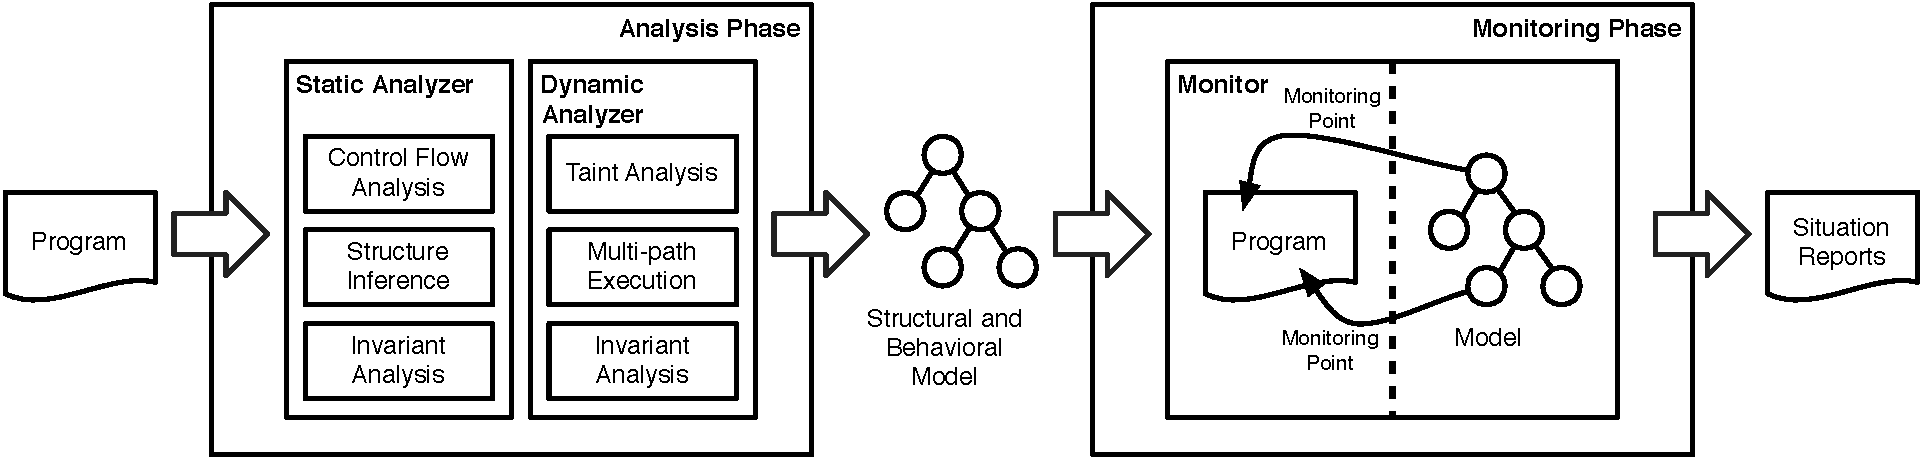
\includegraphics[width=\textwidth]{figures/system-invariants-arch.pdf}
    \caption{Envisioned architecture of the analysis platform.
    A combination of static and dynamic analyses are performed on a replica
    of a deployed system within an isolated, emulated environment.
    The analyses extract a model of high-level program structure and
    legitimate behavior that is then used to monitor the state of the
    deployed system.}
    \label{fig:decomposition-arch}
\end{figure}

\subsection{Dynamic Analysis Engine}

The dynamic analysis engine performs its analysis inside of a high-fidelity
emulated environment based on the \dynamicsys system.  The system monitors the
activity of programs under test during runtime, and has full visibility into
the state of the entire machine at an instruction-level granularity.  This
precision complements the strengths of static analyses; since dynamic analysis
operates over concrete values, the technique has the significant advantage
that it can easily handle obfuscated, self-modifying, and concurrent code.  We
refer the reader to the discussion on \dynamicsys in
Section~\ref{sec:research:firmware} for more details.

In addition to operation over concrete values, we additionally incorporate
dynamic symbolic execution over these traces.  Dynamic symbolic execution
substitutes symbolic values for inputs to individual modules, allowing for the
identification of new inputs that can be provided to the program under test in
order to explore previously uncovered code.  This capability relies upon the
identification of module boundaries and interfaces, which we describe in
Section~\ref{sec:research:structure:modules}.

The output of the dynamic analysis engine is a set of execution traces
augmented with data flow information.  These traces completely describe the
evolution of the state of the program under test with respect to the test
inputs, its interaction with the environment, and the propagation of data
through the system.

\subsection{Static Analysis Engine}

The static analysis engine provides a precise and scalable set of analyses
that operate directly on binary program executables, without the need for
source code.  Incorporating a robust static analysis component allows our
platform to achieve high coverage of program behaviors over possible inputs
without having to actually exercise the program under test on those inputs.
However, static analysis has well-known deficiencies -- especially with
respect to binary executables -- that are important to address.

To that end, we will leverage our prior work on static binary analysis. In
doing so, our platform will be based upon a strong foundation of analyses that
can handle imprecision at multiple levels, including both disassembly and
control flow.

\paragraph{Robust disassembly.} A well-known challenge for binary static
analysis is the difficulty of achieving full coverage of the code contained in
an executable image. Our prior work has studied techniques for improving the
robustness of binary disassembly, and we intend to leverage both symbolic
execution and statistical analysis to that end~\cite{kruegel:sec2004:disasm}.
The use of a symbolic execution engine allows our disassembler to handle many
computed jumps that would otherwise be difficult to resolve statically.

Our work also incorporates statistical techniques to probabilistically
identify likely code regions in binary executables.  An example of this is to
collect, \emph{a priori}, digram probabilities for pairs of instructions from
a corpus of known benign programs.  Then, this can be used during disassembly
to probabilistically identify code regions, or reduce the imprecision
introduced by a (overly-conservative) widened symbolic jump target.

Malicious code also often utilizes obfuscation techniques to hinder static
analysis, such as overlapping instruction sequences as seen in variable length
ISAs such as x86, or switching between multiple supported ISAs as in the case
of ARM and the Thumb family of instruction sets.  We will develop techniques
to handle these classes of obfuscation.

\paragraph{Control-flow subgraph matching.} One capability that is
particularly useful in several contexts relating to binary static analysis is
fuzzy control-flow subgraph matching.  Our prior work has demonstrated its
utility when performing efficient online detection of polymorphic worm
propagation on the network~\cite{kruegel:raid2005:worm}. We anticipate that
this capability will be useful in achieving the goal of module identification
and behavioral characterization.

Our technique for fuzzy control-flow subgraph matching takes two binary CFGs
as input, where graph nodes and edges represent basic blocks and control flow
transfers, respectively.  The algorithm colors the graph based on the
semantics of instructions contained in each basic block, extracts
$k$-subgraphs for small values of $k$ by computing a spanning tree, and then
performs fast subgraph matching to determine the overlap between $k$-subgraphs
from each CFG. By applying abstraction and decomposing the CFGs into
subgraphs, our matching technique is able to efficiently discover
semantically-similar CFGs.  We anticipate that this matching technique can
serve as a robust base upon which to enable module identification.

\subsection{Analysis Capabilities}
\label{sec:research:structure:modules}

The combination of our proposed static and dynamic analyses for binary
programs will enable several key capabilities: automated module
identification, behavioral characterization, interface enumeration, and
runtime monitoring.

\paragraph{Module identification and characterization.} Our composition of
program analyses will allow our platform to automatically identify the
constituent modules of a binary set of programs under test and, in conjunction
with limited \emph{a priori} domain knowledge of the program, classify each
module according to its function.  Module identification will proceed by
iterating between two distinct phases. First, a robust static disassembly and
context-sensitive control-flow analysis will allow our platform to obtain an
initial control-flow graph (CFG) of the program. During this phase,
domain-specific knowledge can be leveraged to statically classify subgraphs of
the CFG as belonging to particular modules -- e.g., by recognizing the
definition and use of interrupt vectors specific to a particular machine
architecture.

During the second phase, this initial static model will be refined by
monitoring the runtime behavior of the program under test.  Ambiguities
resulting from natural limits on the precision of static analysis can be
resolved by observing program behavior over concrete inputs and applying
dynamic symbolic execution over the resulting traces.  For instance,
incomplete coverage of the binary program under test can be improved by
resolving the targets of statically unknown indirect control flow transfers
during the dynamic analysis phase.  The dynamic trace analysis will be
combined with judicious application of novel program invariant inference
techniques~\cite{ernst:2009:daikon,csallner:icse2008:dysy,krka:icsa2010:inference}.
By associating code structure with state invariants at critical program
points, our platform will be capable of recognizing many common program design
patterns of interest.

Iterating between these two phases will allow the platform to identify control
flow patterns that correspond to high-level specifications of expected
behavior defined \emph{a priori} for one or more modules.  For instance, in
the case where a multitasking real-time operating system (RTOS) is being
analyzed, one would expect to observe a control transfer as a result of a
timer interrupt, followed by a deterministic loop over an array or list of
process descriptors, followed by the resumption of a selected thread of
control.  Our platform will allow for the specification and matching of such
high-level patterns of control flows against real binaries and execution
traces.  In the case that concurrent execution of multiple modules is
encountered by the platform, domain-specific knowledge will be leveraged for
the particular machine architecture to isolate and extract traces for each
distinct thread of execution.

\paragraph{Invariant analysis.} Prior work on invariant analysis major
limitations that we aim to improve in our proposed work.  First, current
invariant invariant approaches are primarily limited to either predefined
templates~\cite{ernst:2009:daikon} or extraction of low-level invariants from
program code~\cite{csallner:icse2008:dysy}.  While extraction of low-level
invariants is a promising direction, we will develop techniques for inferring
high-level invariants over module behavior and inter-module communication in
the context of high-level module behavior summaries that are security-relevant
-- i.e., useful for enforcing security properties such as isolation between
   modules with different privilege levels or belonging to distinct security
   principals.

A second limitation of current invariant detection approaches is that they
require either source code, bytecode, or binary programs compiled with
debugging information.  In our work, we aim to extend invariant analysis to
cover binary programs for which we do not have access to such information.
This will require differential analysis of the memory of the program during
execution at selected program points.  In addition, we will define algorithms
to scope the differential program state analysis to the subset of memory that
can be accessed by the current region of code -- e.g., the currently executing
function.  Determining this memory subset will require incorporation of both
static and dynamic information.

Finally, we aim to address the restriction that current invariant analyses are
primarily limited to the form of pre- and post-conditions on function or
method invocations.  A major part of our work will include the identification
and application of invariants in a fine-grained manner, where we will select
critical points in the CFG using structural analysis to apply our invariants.
As an example, using this approach we aim to discover program points such as
loops over critical data structures, or switch tables that correspond to
individual protocol state handlers

\paragraph{Module interface enumeration.} Once a set of modules has been
identified from the combination of the statically-derived CFG and runtime
monitoring, the analysis platform will proceed to automatically identify the
interfaces exposed by each module.  This step will take into account
domain-specific knowledge regarding machine architecture -- e.g., to identify
the use of special instructions that allow for control transfers between
modules such as system call service invocations.  To enable richer semantic
understanding of not only the vectors for entering a module, but also the
types of data that accompanies these control transfers, the platform will
leverage a combination of static and dynamic data-flow analyses to
characterize the number and types of parameters for control transfers across
modules.  In cases where memory is shared between modules, points-to analyses
will be leveraged to characterize the data shared between modules and the sets
of modules that contain references to particular memory objects.  For
instance, returning to the example of an RTOS, our platform will be able to
identify well-known structures such as process lists or memory descriptors as
channels of information flow that serve as an \emph{implicit} interface
between logically-distinct modules.

\paragraph{Runtime monitoring.} The result of the previous phase will be a
high-level structural model of the system under test in the form of a
decomposition of independent models, a characterization of their function and
behavior, and execution state invariants at critical program points.  This
model will then be used by a runtime component that will monitor the execution
of the deployed system. The monitoring component will use dynamic state
introspection and will be protected from attacks against integrity using a
robust isolation mechanism. Introspection will occur at carefully selected
program points in order to balance behavioral coverage with performance
requirements.

Deviations from the model that are indicative of anomalous and potentially
malicious factors will be detected and reported.  Additionally, due to the
characterization analysis performed during model construction, reports will
contain high-level information concerning \emph{why} the observed behavior is
anomalous, leading to increased whole-system insight on the part of system
analysts and operators.

\section{Summarizing Software Execution}
\label{sec:research:autosummary}

Existing work on reverse engineering binary code has typically focused
on decompilation~\cite{schwartz:2013:decomp,cifuentes:1995:decomp}.
However, for quickly understanding the behavior and capabilities of a
program, source code may not be the most efficient representation.
Instead, one may desire \emph{semantically meaningful summaries} of
parts of a program or execution trace. For example, portions of an
execution might be summarized as ``argument parsing'',
``serialization'', or ``encryption''.

This kind of high-level labeling is often performed implicitly by human
reverse engineers as they analyze a program. One may glance over the
functions in a binary to get a rough idea of their purpose before
deciding where to spend one's (limited) analysis time. We propose to
build a system that can quickly provide these kinds of high-level
semantic summaries \emph{automatically}. 

To accomplish this, we propose to look to the area of streaming
analytics. Previous work from Georgia Tech~\cite{dolangavitt:2013:tzb}
has demonstrated that viewing a program execution as a large number of
streaming memory accesses, combined with an analysis of the contents of
these streams, can be a powerful tool for program explication. This
notion can be extended beyond memory accesses to other artifacts of
computation, effectively treating an execution as a generator for
streams of observations of the program's state. By collecting statistics
on these streams and comparing them to a corpus of labeled exemplars, we
will be able to classify execution fragments according to high-level
semantic descriptions.

\subsection{Programs as Streaming Data}

To perform a high-level labeling, we need to generate a set of
observations about the behavior of portions of program execution both in
the training corpus and for new executions we wish to understand. In
previous work~\cite{dolangavitt:2013:tzb}, this took the form of streams
of data from memory accesses. In our proposed system, we will augment
these with a number of other observables, for example:

\begin{itemize}
    \item System, API, and function calls
    \item CPU register contents over time
    \item Assembly instruction mnemonics in a sliding window over the
    instruction stream
    \item Externally visible outputs such as disk, network, and IPC
\end{itemize}

Each of these can be combined with its context within the program (i.e.,
the module as identified by our structural decomposition and the calling
context) to break up these data streams. The key idea is that these
sub-streams will now contain data that is of the same semantic type, as
each is generated from within the same part of the program. Taken
together, the content of these streams should thus form a fingerprint
for the code's functionality. Some streams may be noisier than others,
but creating robust classifiers from noisy signals is a well-studied
problem in machine learning.

\subsection{Creating a Labeled Corpus}

A natural approach to creating a labeled corpus of program functionality
is to manually examine many programs and assign meaningful labels to
their various components. Aside from the daunting amount of work this
would require to build a reasonably-sized corpus, this strategy is also
inherently underspecified. Any labeling effort would need to decide
\emph{a priori} on a consistent set of labels, but the diversity of
real-world program behaviors means any such label set would likely be
incomplete.

Instead we propose to generate our corpus from precisely the semantic
information that is usually removed during compilation: comments and
variable names. Naturally, these labels will not be as precise as those
a human would create, but in aggregate they should provide valuable
information on the meaning of the code in question.

Thus, to create a corpus one can start by compiling a large number of
open source programs with debugging information. The resulting binary
code can then be given labels derived from the comments and variable
names. Finally, the programs can then be run in \dynamicsys to create
the streams of observations that will be used in classification.

\subsection{Classifying Execution Fragments}

Given a new execution, we can now generate the same streams of
observations as for the exemplar corpus. These observations can then be
matched against the models generated in training to find those that most
closely match. The output is a labeled instruction stream that assigns
\emph{meaning} to execution fragments.

This problem can also be seen as a statistical machine translation
problem with three parallel corpora: the comments and variable names in
the code, the binary code produced from compilation, and the streams of
observations produced by running the code. The first two are explicitly
related via the source code to binary mapping produced by compilation.
The latter two can be seen as implicitly related by some noisy channel. 
Using techniques from machine translation, we can find a mapping between
the first and third, giving us the desired semantic labeling.


\section{Encrypted Protocol Fuzzing}
\label{sec:research:fuzzing}

Fuzz testing or fuzzing has been widely used in software vulnerability
discovery. The basic idea behind fuzzing is to generate a large number
of malformed inputs by either mutating normal inputs or directly
constructing them according to predefined generation rules, and then use
the malformed inputs to test the target software. Despite the simplicity of
the concept, fuzzing has proven very effective in uncovering previously
unknown vulnerabilities in complex software. However, existing fuzzing
technologies are hardly applied to undocumented and encrypted protocols,
because the generated inputs do not satisfy integrity validation checks or
become meaningless after being decrypted and are dropped.

For example, many instant messengers (IM) encrypt all network
traffic for privacy protection. In this case, upon receiving a message,
such an IM client would verify the integrity of the message, decrypt the
payload of the message, and further handle the decrypted data.  In
comparison with the code responsible for integrity verification and
message decryption, the code responsible for handling decrypted data is
usually more vulnerable. Unfortunately, without knowing the IM protocol,
network-fuzzing tools cannot construct a meaningful message that can
reach the most vulnerable region.

We propose to develop a smart fuzzing platform based on the
\dynamicsys system and the module identification analysis, with the goal
of coping with encrypted network protocols and improving the effectiveness
of fuzzing.  Our intuition is that in order to support
bidirectional communication, the programs (such as IM clients) capable
of decrypting messages usually own the encryption capability at the same
time.  By using dynamic data flow tracking and the module identification
analysis, we expect to identify the modules in a program that are
responsible for message encryption and decryption. As a result, rather
than constructing a malformed network packet from scratch, we
propose to leverage the program themselves to build syntactically
correct but semantically incorrect data and then use the data to test
the programs.

Consider the case of IM clients as a concrete example.  After two IM clients
initialize a communication channel, we can introduce data mutation to the
input buffer of the encryption function at runtime on one side and then send
the encrypted message to the other side. In this case, the encrypted message
would be completely accepted by the other side and reach a region of code that
is more likely to be vulnerable.  Furthermore, during the process of how the
IM client handles a correctly decrypted message, we can apply the dynamic data
flow tracking technique to identify the input bytes that flow into security
sensitive operations, meaning they are more likely to trigger vulnerabilities.
Then we use this knowledge to guide the data mutation.


\section{Broader Impact and Educational Outreach}
\label{sec:impact}

The lack of insight into closed-source software such as embedded firmware and
commercial applications limit the abilities of security analysts and tools to
detect malicious behavior and harden vulnerable software.  The techniques and
tools developed by this project will help to remedy this situation, by
giving specialists and organizations the necessary capabilities to perform
these tasks.  Since such software is pervasive in the modern Internet and
within targeted organizations, the results of this project will result in
safer systems and a more secure Internet.

\subsection{Curriculum Development}
\label{sec:impact:curriculum}

The novel research to be performed as part of this project will have a direct
impact on the undergraduate and graduate curricula of Northeastern University
and the Georgia Institute of Technology.  PIs Kirda and Robertson are both
directly responsible for teaching efforts in systems and network security at
Northeastern, and will directly transfer the knowledge gained in the course
of this project to the classroom.  PI Wang is similarly well-placed to ensure
that this research will enrich the security curriculum at Georgia Tech.

Outside of the classroom, both institutions are deeply involved in practical
educational efforts in security -- e.g., Capture-the-Flag (CTF) competitions --
that help to train students and outside participants in real-world security
tools and techniques.  The results of this research will also inform these
efforts.

\subsection{Education and Outreach}
\label{sec:impact:education}

Aside from curriculum development, all PIs are actively engaged in many
collaborations within the wider security community, including other academic
groups, industry, and the government.  As such, the research performed in this
project will enjoy wide dissemination through this network in the form of
collaborations, talks, published papers, and scientific visits.

\section{Project Time Plan}
\label{sec:time-plan}

Work on the proposed project will adhere to the following annual schedule.
With each goal, we will aim to publish our results in top- tier systems
security venues, and publicly release our prototypes and data -- in accordance
with our data management plan -- for testing and adoption by the community.

\paragraph{Year 1.} The primary goal of the first year will be to adapt our
prior work on emulation-based dynamic analysis to scale to entire systems in
support the subsequent work to be performed as part of this project. We will
also define and enumerate the low-level features we will use in this project
to infer software and system module boundaries in closed-source software, as
well as whole-system behavioral summaries. Additionally, we will begin the
integration into the framework of our static analysis engine and dynamic
symbolic analyzer to support the extraction of behavioral models.  Finally, we
will collect a representative sample of binary program artifacts to evaluate
our techniques against.

\paragraph{Year 2.} In the second year, we will continue to develop the
analysis framework, concentrating on researching novel techniques for behavior
summarization and structural inference.  In particular, we will focus on
extending the state of the art in dynamic invariant learning.  We will also
begin applying the techniques and analysis framework to applications such
as the proposed encrypted protocol fuzzing approach.

\paragraph{Year 3.} The final year of the project will include further
development of the analysis platform.  In particular, we will incorporate
techniques for automated enforcement of learned normal behavior defined by
inferred invariants and behavioral models.  We will also investigate other
applications of the whole-system dynamic analysis framework for securing
closed-source systems.

\section{Qualifications of the PIs and Previous NSF Support}
\label{sec:qualifications}

\paragraph{Engin Kirda} is an Associate Professor at the College of Computer
and Information Science and the College of Engineering at Northeastern
University. PI Kirda has published extensively in the area of systems
security. Before moving to the Northeastern University in 2011, Dr.~Kirda has
held faculty positions at Institute Eurecom in France and Technical University
of Vienna in Austria. At Northeastern, he is the holder of the Sy and Laurie
Sternberg Chair in Information Assurance, and also the director of the
Northeastern Information Assurance Institute. His research to date has focused
on malware analysis and detection~\cite{bayer:ndss2009:malware,kirda06:bho,kolbitsch10:gadget,moser:ssp2007:malware,yin07:panorama},
web application security~\cite{kirda10,mcallister2008}, and recently,
the human aspects of cyber security~\cite{onarlioglu12,irani11,balduzzi10:raid,bilge09:social,wondracek10:deanon}.
He has co-authored more than 90 peer-reviewed scholarly publications and served on
program committees of numerous well-known international security conferences
and workshops. In 2009, Dr.~Kirda was the Program Chair of the International
Symposium on Recent Advances in Intrusion Detection (RAID), in 2010/11,
Program Chair of the European Workshop on Systems Security (Eurosec), and was
the Program Chair of the USENIX Workshop on Large Scale Exploits and Emergent
Threats in 2012. Dr.~Kirda will be chairing the top-tier conference NDSS in
2015. PI Kirda's research has also been frequently covered by the popular
press. In 2012, he led a congressional briefing on emerging cyber threats.

PI Kirda moved to the U.S.~in 2011, and is currently the PI of the recent NSF
grant CNS-1116777, {\em Automatically Identifying Botnet Command and Control
Infrastructures} (2011--2014).  This grant aims to develop novel techniques
and tools to detect malicious connections from compromised machines to the
command and control servers of botnets. The goal of the project is to build a
detection prototype called DISCLOSURE. This grant has already resulted in
well-known publications and systems~\cite{acsac2012disclosure,issta2012malware}.

\paragraph{William Robertson} is an Assistant Professor at the College of
Computer and Information Science and the College of Engineering at
Northeastern University.  His research interests revolve around web security,
program analysis, anomaly detection, and trustworthy computing architectures.
He was involved in both the California Top-to-Bottom-Review (TTBR) and the
Ohio EVEREST projects as a Red Team member.  In this capacity, he demonstrated
that electronic voting systems were potentially susceptible to large-scale
attacks that could exploit numerous vulnerabilities in the firmware and
physical security of the components of the voting system.  These findings led
to significant changes in public policy in both states with respect to
electronic voting, including restrictions or outright bans on the use of these
systems.  He is also involved in Lastline, Inc., a startup focused on
detecting advanced persistent threats and zero day attacks that is in part
based on his academic work.

PI~Robertson also has extensive experience in organizing and participating in
Capture-the-Flag (CTF) exercises.  With Shellphish, a team composed of
UCSB-affiliated members, he won the 2005 edition of the DEFCON CTF
competition.  He was also instrumental in helping to organize the UCSB iCTF,
the largest distributed CTF competition, from its inception in 2003 to 2008.

PI~Robertson was the program chair of the 2013 USENIX Workshop on Offensive
Technologies (WOOT), co-located with USENIX Security.  He was the chair of the
2012 Conference on the Detection of Intrusions and Malware \& Vulnerability
Assessment (DIMVA).  He has participated on the program committees of a number
of top-tier systems security venues, including IEEE Security and Privacy,
USENIX Security, and RAID.  He is also the author of more than twenty
peer-reviewed journal and conference papers in the area of systems and network
security.

PI~Robertson is currently the PI of an NSF SFS award entitled
``Multi-Disciplinary Preparation of Next Generation Information Assurance Practitioners''
that seeks to train the next generation of cybersecurity professionals for
service in U.S.~government agencies.

\paragraph{Tielei Wang} is a research scientist in the Department of Computer
Science at the Georgia Institute of Technology.  His research interests include
systems and software security, with an emphasis on advanced attack and defense
techniques, including software vulnerability detection and exploitation.  He
has developed both static and dynamic software vulnerability detection systems,
and has discovered a number of zero day vulnerabilities in software products
from Microsoft, Adobe, Google, Yahoo, IBM, and Apple.  He is a recipient of
the 2010 IEEE Symposium on Security and Privacy (Oakland'10) best student
paper award, 2011 China Computing Federation (CCF) distinguished doctoral
dissertation award, and 2011 Secunia most valued contributor award.

He served on the program committee of the 32nd IEEE International Performance
Computing and Communications Conference, and the the 14th International
Workshop on Information Security Applications.

PI Wang has net yet received NSF support.

\newpage
\pagenumbering[E]{bychapter}
\setcounter{page}{1}
\setcounter{section}{0}
\bibliographystyle{acm}
\bibliography{satc}

% \newpage
% \pagenumbering[F]{bychapter}
% \setcounter{page}{1}
% \setcounter{section}{0}

\end{document}
